\documentclass[twocolumn,amssymb,prb,aps,superscriptaddress]{revtex4}

\usepackage{graphicx}
\usepackage[utf8]{inputenc}
\usepackage{amsmath}
\usepackage{float}


\begin{document}

\begin{abstract}
    Hola Abstract, este es un pequeño resumen del documento presentado
\end{abstract}

\title{Resonancia Paramagnetica Spin Electrón}
\author{Majo}

\affiliation{Colegio de Ciencias e Ingeniería, USFQ, Quito, Ecuador} 

\author{Martin}

\affiliation{Colegio de Ciencias e Ingeniería, USFQ, Quito, Ecuador}

\date{\today}

\maketitle

\section[Intro]{Introducción}
\label{sec:intro}

Lo que es, de donde sale, quien lo descubrio, lo que dice en wikipedia y que vamos a decir en paper

\section[]{Cuántica del Sistema}
\label{sec:cuantica}
El prototipo basico de RPE es una interaccion entre 2 particulas de Spin $1/2$, el proton del nucleo con spin $\vec{I}$ y el del $e^-$ $\vec{S}$. El hamiltoniano del sistema electron nucleo puede escribirse con terminos de la interacción entre los 2 spines $ \vec{I} \cdot \vec{S} $ y los terminos de Zeeman $g \beta \vec{H} \cdot \vec{J}$, si asumimos que el $\vec{H}$ esta en $z$ tenemos

\begin{equation}
    \label{eq:hamiltonianoDelSistema}
    \mathcal{\hat{H}} = H (g_e \beta \hat{S_z} - g_N \beta_N \hat{I_z}) + T \vec{S} \cdot \vec{I} 
\end{equation}

\subsection{Momentos Angulares y Spines}
\label{sec:momentosAngulares}

\subsection{interacción Spin Campo}

\subsection{Estadistica del sistema}
\label{mecanicaEstadistica}

    \begin{figure}[H]
        \centering
        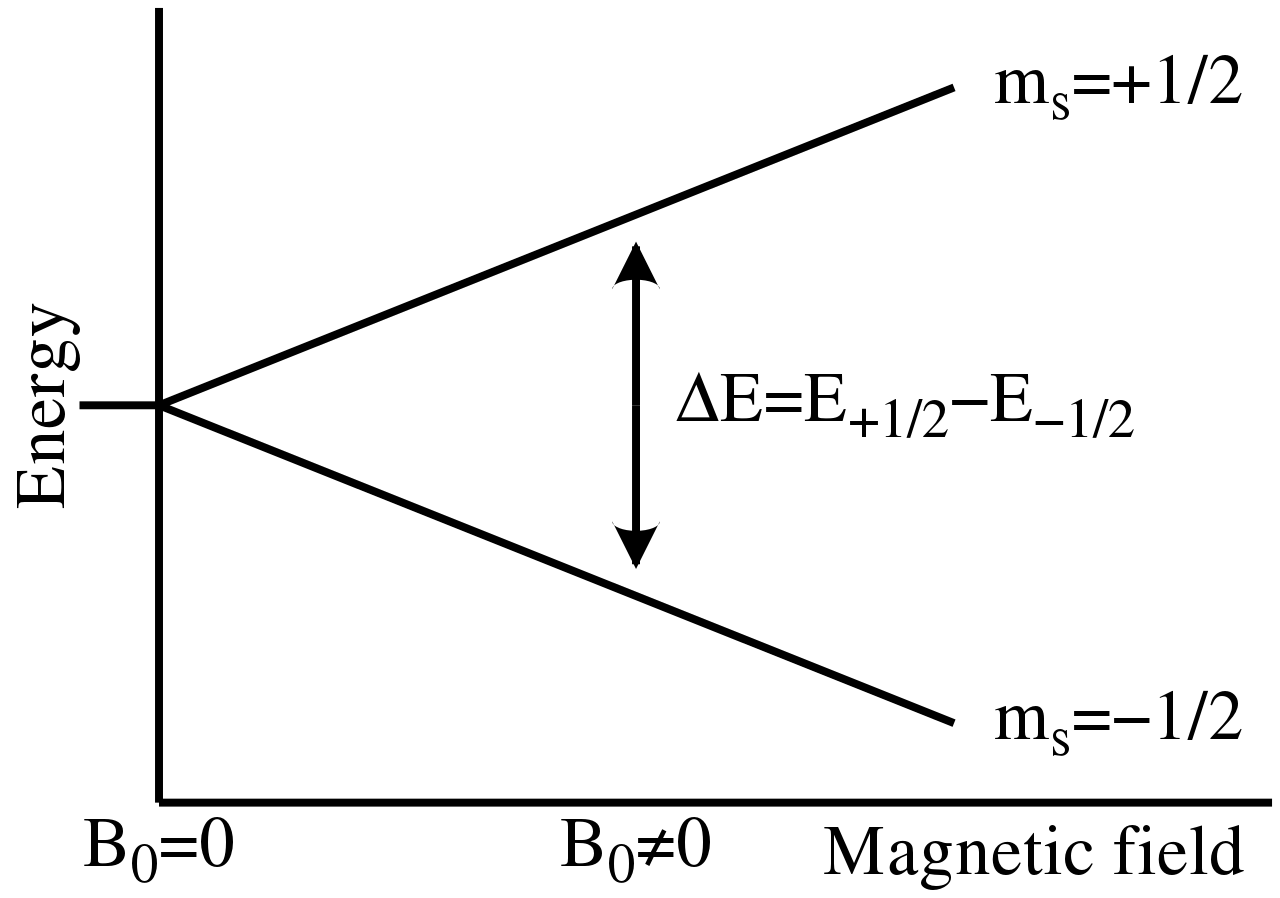
\includegraphics[width=6.0cm]{images/EPR_splitting}
        \caption{Diagrama de diferencia de Energia}
        \label{fig:diagramaDiferenciaDeEnergia} 
    \end{figure}

\section{Aplicaciones}
\label{sec:aplicacion1}

\subsection{Espectroscopia}
\label{sec:aplicacion2}

\subsection{Metales}

\subsection{Datacion}

\end{document}